\documentclass[10pt,a4paper]{article}
\usepackage[utf8]{inputenc}
\usepackage[french]{babel}
\usepackage[T1]{fontenc}
\usepackage{amsmath}
\usepackage{amsfonts}
\usepackage{amssymb}
\usepackage{graphicx}
\usepackage[colorlinks = true,
            linkcolor = blue,
            urlcolor  = blue,
            citecolor = blue,
            anchorcolor = blue]{hyperref}
\title{Apprentissage profond par renforcement \\ Compte-rendu de TP}
\author{Nelly Barret et Juliette Reisser}

% code
\usepackage{listings}
\usepackage{xcolor}
\definecolor{codegreen}{rgb}{0,0.6,0}
\definecolor{codegray}{rgb}{0.5,0.5,0.5}
\definecolor{codepurple}{rgb}{0.58,0,0.82}
\definecolor{backcolour}{rgb}{0.95,0.95,0.92}
\lstdefinestyle{mystyle}{
    backgroundcolor=\color{backcolour},   
    commentstyle=\color{codegreen},
    keywordstyle=\color{magenta},
    numberstyle=\tiny\color{codegray},
    stringstyle=\color{codepurple},
    basicstyle=\ttfamily\footnotesize,
    breakatwhitespace=false,         
    breaklines=true,                 
    captionpos=b,                    
    keepspaces=true,                 
    numbers=left,                    
    numbersep=5pt,                  
    showspaces=false,                
    showstringspaces=false,
    showtabs=false,                  
    tabsize=2
}
\lstset{style=mystyle}

% subsubsubsection
\usepackage{titlesec}

\setcounter{secnumdepth}{4}

\titleformat{\paragraph}
{\normalfont\normalsize\bfseries}{\theparagraph}{1em}{}
\titlespacing*{\paragraph}
{0pt}{3.25ex plus 1ex minus .2ex}{1.5ex plus .2ex}


\begin{document}
\maketitle

\section{Préliminaires}
Notre TP se trouve à l'adresse suivante : \href{https://github.com/NellyBarret/IA5-TP-APR}{https://github.com/NellyBarret/IA5-TP-APR}

Nous avons principalement utilisé les libraires suivantes :
\begin{itemize}
	\item \href{https://gym.openai.com/}{Gym} pour les environnements d'apprentissage
	\item \href{https://keras.io/}{Keras} (de Tensorflow) pour les modèles de réseaux neuronaux
	\item \href{https://numpy.org/}{Numpy} pour les calculs
	\item \href{https://matplotlib.org/index.html}{Matplotlib} pour les tracés de courbe
\end{itemize}

%TODO : logique générale
Nous allons d'abord définir quelques variables communes aux différentes implémentations. Ces variables font partie de la logique même utilisée par Gym.

Nous avons accès à deux variables importantes quant à la définition de l'environnement :
\begin{itemize}
	\item \lstinline{env.action_space} qui définit les actions possibles pour l'agent. Chaque action est un entier, e.g. 0 pour aller à gauche, 1 pour aller à droite.
	\item \lstinline{env.observation_space} qui définit un tableau représentant les métriques importantes de l'environnement, e.g. la position d'un élément, les frames d'un jeu...
\end{itemize}

Nous avons aussi 3 variables importantes quant à l'exécution d'actions sur l'environnement :
\begin{itemize}
	\item \lstinline{next_state} qui définit le nouvel état (après exécution de l'action sur l'environnement)
	\item \lstinline{reward} représente la récompense gagnée par l'agent après exécution de l'action sur l'environnement
	\item \lstinline{done} est un booléen pour indiquer si l'épisode courant est fini (i.e. le bâton est tombé ou sorti de l'environnement)
\end{itemize}

Enfin, nous avons deux méthodes importantes quant à la communication environnement/agent :
\begin{itemize}
	\item \lstinline{act()} qui retourne l'action choisie par l'agent. C'est dans cette fonction que nous implémenterons les politiques (de sélection d'action), i.e. aléatoire, $\epsilon$-greedy et Boltzmann. 
	\item \lstinline{step(action)} qui exécute une action sur l'environnement et retourne les 3 variables expliquées ci-dessus. 
\end{itemize}

\section{Deep Q-network sur Cartpole}

\subsection{Début}

\subsubsection{Question 1}

Fichier correspondant : \href{https://github.com/NellyBarret/IA5-TP-APR/blob/master/randomCartPole.py}{randomCartpole.py}

\paragraph{Définition de l'environnement}

Dans l'environnement CartPole (variable \lstinline{env}), nous avons un bâton posé en équilibre sur un élément que l'on peut faire bouger à gauche ou à droite pour rééquilibrer le bâton. L'objectif principal pour l'agent est de maintenir le bâton assez vertical pour que celui-ci ne tombe pas et/ou ne sorte pas de l'environnement.

Nous avons accès à deux variables importantes quant à la définition de l'environnement :
\begin{itemize}
	\item Ici, l'espace des actions est de taille 2 car l'agent peut faire bouger l'élément à gauche (action 0) ou à droite (action 1).
	\item L'espace des états est de taille 4 car il est défini comme suit : [position de l'élément, vitesse de l'élément, angle du bâton, taux de rotation du bâton]
\end{itemize}


Enfin, nous avons deux méthodes importantes quant à la communication environnement/agent :
\begin{itemize}
	\item \lstinline{act()} utilise une politique aléatoire
	\item \lstinline{step(action)} 
\end{itemize}

\paragraph{Définition de l'agent}

L'agent aléatoire suit une politique aléatoire pour choisir l'action qu'il va exécuter dans l'environnement. Il les choisit parmi ses actions possibles (disponibles dans \lstinline{env.action_space}). L'agent aléatoire choisit simplement des actions des manière aléatoire puis les exécute sur l'environnement.

\begin{lstlisting}[language=Python, caption=Programme principal de l'agent aléatoire]
# (1)
env = gym.make("CartPole-v1")
agent = RandomAgent(env.action_space)

# (2)
nb_episodes = 100

# (3)
for i in range(nb_episodes):
    state = env.reset()
    # (4)
    while True:
        action = agent.act() # (5)
        _, reward, done, _ = env.step(action) # (6)
        if done: # (7)
            break
    env.close()
\end{lstlisting}


\textbf{\textsc{Partie code:}}
\begin{lstlisting}[language=Python]
# (1)
\end{lstlisting}
Nous créons un environnement Gym avec comme paramètre le nom de l'environnement à créer. Nous créons ensuite notre agent aléatoire. Celui-ci redéfinit les méthodes suivantes :
\begin{itemize}
	\item \lstinline{act()} : cette méthode renvoie une action parmi les actions possibles
	\item \lstinline{sample()}. La p
\end{itemize}

\begin{lstlisting}[language=Python]
# (2)
\end{lstlisting}

\begin{lstlisting}[language=Python]
# (3)
\end{lstlisting}

\begin{lstlisting}[language=Python]
# (4)
\end{lstlisting}

\begin{lstlisting}[language=Python]
# (5)
\end{lstlisting}

\begin{lstlisting}[language=Python]
# (6)
\end{lstlisting}

\begin{lstlisting}[language=Python]
# (7)
\end{lstlisting}

\subsubsection{Question 2}

Fichier correspondant : randomCartpole.py

Pour évaluer l'agent, nous avons réalisé un graphique traçant la somme des récompenses obtenues pour chaque épisode.

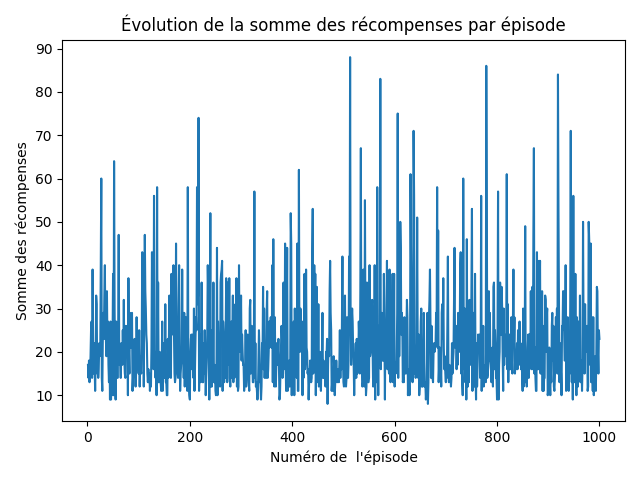
\includegraphics[scale=0.5]{evolution_recompenses_random.png} 

Nous pouvons observer qu'il n'y a pas de tendance particulière. Cela semble cohérent avec le fait que l'agent n'a aucun moyen d'apprendre de ses erreurs (pas de mémoire ni de rétro-propagation) et qu'il ne choisisse pas les meilleures actions (politique aléatoire).

\subsection{Experience replay}

\subsubsection{Questions 3 et 4}

Fichier correspondant : ExperienceReplayAgent.py

Dans cet agent, nous avons d'abord créé un objet Memory qui représente la mémoire de l'agent. Cette mémoire stocke les informations (i.e. expériences) sous la forme d'un tableau d'éléments : 
$$ [state, action, reward, next_state, done] $$
Le tableau de toutes ces expériences représente la mémoire de l'agent.

Sur cette mémoire, nous avons principalement deux fonctions :
\begin{itemize}
	\item \textit{L'ajout d'une nouvelle expérience} : cette fonctionnalité permet à l'agent de se souvenir de ce qu'il vient d'expérimenter dans l'environnement. Comme la mémoire a une taille limitée, le nouveaux éléments remplacent les anciens quand celle-ci est pleine.
	\item \textit{La création d'un batch} : cette fonctionnalité permet de choisir des éléments de manière aléatoire dans la mémoire et de retourner ce batch d'expériences.
\end{itemize}

\subsection{Deep Q-learning}

\subsubsection{Question 5}

\subsubsection{Question 6}

\subsubsection{Question 7}

\subsubsection{Question 8}

\section{Breakout Atari}

\subsubsection{Question 1}

\subsubsection{Question 2}

\subsubsection{Question 3}

\subsubsection{Question 4}

\subsubsection{Question 5}
\end{document}